% Part 3 opening chapter: one gauge across the applications (the quantum-processor report, the semiconductor report, the methylation report).
% Built 2026-10-02 from the author's saved excerpt (this conversation, 2026-09-30, archive messages 17511, 17523, 18385, 18409, 18492),
% updated to the master table v1.1 (CANON/iam_canon.json, 2026-10-02): per-cell H_min (class H_min retired 2026-10-01), M = E/k_BT = 20.94,
% one meaning for A, law first (the virial partition is an application, not an expression of the law). Symbols: Appendix~\ref{app:canon}.
\chapter{One gauge: the reading over its floor}\label{ch:onegauge}

\section*{The place}
IAM's Law (Chapter~\ref{ch:iams_law}): every irreversible transition from quantum superposition to classical record pays $k_BT\ln2$ per bit to
the nearest encoding surface, at that surface's temperature. A switching transistor, a measured qubit and a copied methylation mark are all
records written against thermal noise. The applications in this part read each of them the same way: the measured record over the lowest
record the system allows at its temperature. Thermal noise is not filtered out; it is the yardstick.

\section{The symbols}
\begin{center}\small\begin{tabular}{p{0.11\textwidth}p{0.36\textwidth}p{0.45\textwidth}}\toprule
symbol & meaning & in every domain\\\midrule
$H_{\min}$ & the floor & the lowest reading the system allows, measured on the same instrument\\
$A$ & reading$/H_{\min}$ & dimensionless; $A=1$ is the floor (cells: the healthy cell's own floor)\\
$M$ & $E/k_BT$ & drive energy over the thermal noise quantum; $M/\ln2$ in Landauer units\\
$n$ & temperature exponent & $A(T)=A(T_{\rm ref})(T/T_{\rm ref})^n$; calibrated per class, never derived, never $A$\\\bottomrule
\end{tabular}\end{center}
\begin{center}\small\begin{tabular}{p{0.13\textwidth}p{0.27\textwidth}p{0.25\textwidth}p{0.25\textwidth}}\toprule
domain & reading & $H_{\min}$ & $A$\\\midrule
chips (the semiconductor report) & $E_{\rm sw}=\mathrm{TDP}/(N f)$ & Landauer floor $k_BT_j\ln2$ & $E_{\rm sw}/(k_BT_j\ln2)$; $M=A\ln2$\\
qubits (the quantum-processor report) & $\varepsilon=-\ln(1-p_{2Q})$ & material floor $\varepsilon_{\rm floor}$ (calibrated) & $\varepsilon/\varepsilon_{\rm floor}$\\
cells, arrays (Met-A) & mean $H(\beta)$ over identity sites & the cell type's reference floor & Met-A\\
cells, molecules (IAM-A) & $H(\varepsilon)$, copy error & $P_{\rm cell}\,H(\varepsilon_0)$ & IAM-A\\\bottomrule
\end{tabular}\end{center}
For a chip the floor is the law itself. For a qubit it is a property of the substrate. For a cell it is the healthy cell of the same type, read
on the same platform (Met-A), or the physics floor at the cell's frozen position (IAM-A). Example: the AMD Ryzen 9 9950X (170\,W, $20.6\times10^9$
transistors, 4.3\,GHz, $T_j=75\,^\circ$C) switches at $E_{\rm sw}=1.92\times10^{-18}$\,J, $576$ times the Landauer floor, $M=399$.

\paragraph{One gauge, each domain in its own form.} Every $A$ is an error score read on the same gauge (Fig.~\ref{fig:onegauge}): the reading
divided by the same system's healthy reading, so that $A=1$ is the system working as itself and sits in the middle. Below it lies $H_{\min}$, the
absolute lowest error the system can hold before thermal kicks win; nothing reads below $H_{\min}$. Above 1 the system makes more error than when
healthy. The formula is not the same in every domain, and should not be: the error comes from different physics in each (laser and motional noise in a
trapped ion, Rydberg decay in a neutral atom, two-level fluctuators in a transmon's oxides, thermal emission in a hot molecule, a missed site at DNA
replication), and each field writes its thresholds in its own units.
\begin{center}\small\begin{tabular}{p{0.12\textwidth}p{0.25\textwidth}p{0.23\textwidth}p{0.3\textwidth}}\toprule
score & reading & healthy reference ($A=1$) & $H_{\min}$ (on the gauge)\\\midrule
IAM-A & copy error, $H(\varepsilon)$ & $P_{\rm cell}H(\varepsilon_0)$ & $H(\varepsilon_0)$; neutrophils at $1/P=0.910$\\
Met-A & $\langle H(\beta)\rangle$ at identity sites & purified healthy cells, same platform & not yet derived for arrays\\
C-score & clustering of the residual map & healthy median clustering & ---\\
the quantum-processor report & $\varepsilon=-\ln(1-p_{2Q})$ & the device as built & material floor (Helios: $0.13$)\\
the semiconductor report & $E_{\rm sw}=\mathrm{TDP}/(Nf)$ & the chip as built & Landauer floor $k_BT_j\ln2$ (9950X: $0.0017$)\\\bottomrule
\end{tabular}\end{center}
Some systems also have a point on the high side where they stop working: for a qubit, the gate error at which error correction fails ($p\approx1\,\%$;
Helios at $A=12.7$). For cells the high side is the cancer direction; no failure point has been measured. The region between $H_{\min}$ and the healthy
band is less error than healthy; for cells what it means biologically has not yet been measured.

\begin{figure}[h]\centering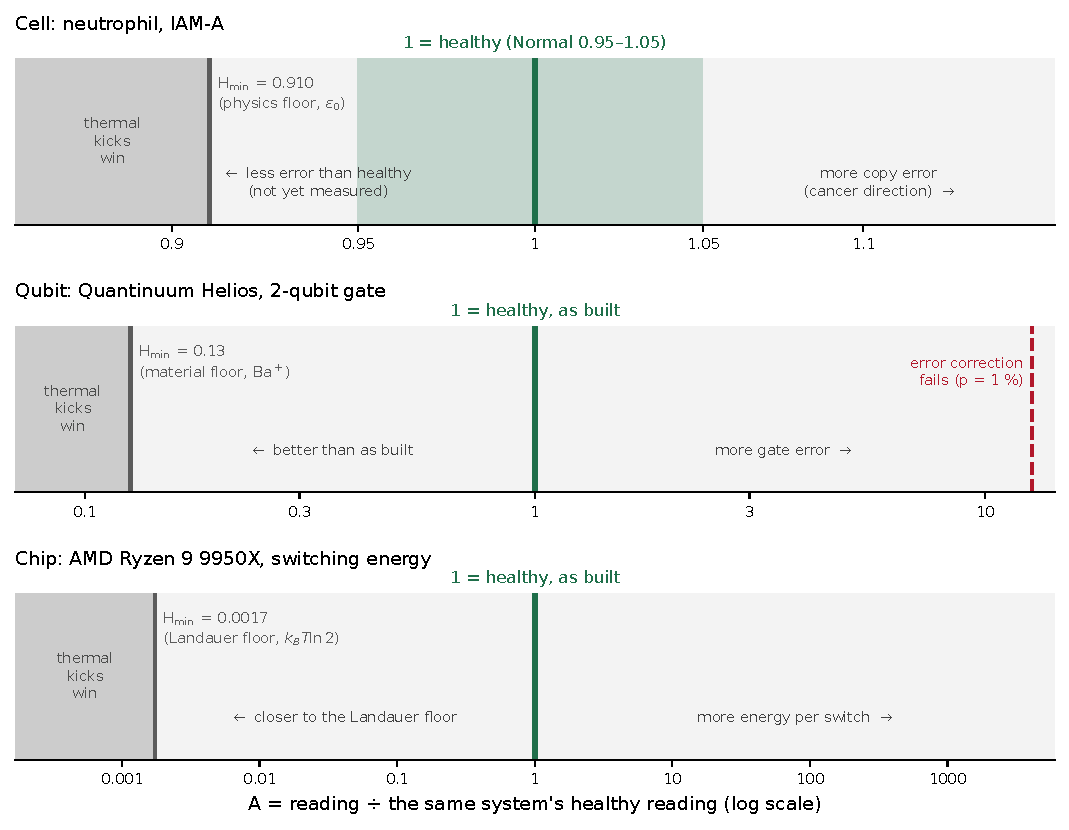
\includegraphics[width=\textwidth]{figs_one_gauge/one_gauge.pdf}
\caption{One gauge for every score. $A=1$ is the healthy reading of that same system (green); $H_{\min}$ (grey line) is the lowest error it can hold
before thermal kicks win, and nothing reads below it (grey zone). Cell: neutrophil IAM-A, $H_{\min}=H(\varepsilon_0)$ at $1/P_{\rm cell}=0.910$, Normal
band 0.95--1.05. Qubit: Quantinuum Helios two-qubit gate ($p=7.9\times10^{-4}$) against a Ba$^+$ material floor of $10^{-4}$ (calibrated); error
correction fails near $p=1\,\%$. Chip: AMD Ryzen 9 9950X (170\,W, $20.6\times10^9$ transistors, 4.3\,GHz, $T_j=75\,^\circ$C) against the Landauer floor.
Each row has its own log scale, centred on 1.}\label{fig:onegauge}\end{figure}

\paragraph{Where $H_{\min}$ comes from.} For the cell, the form of the floor is IAM's Law: a holding energy $E_{\rm hold}$ against $k_BT$ allows
an error $\varepsilon_0=1/(1+e^{E_{\rm hold}/k_BT})$. Its height is at present measured: $E_{\rm hold}=\varphi M=3.41\,k_BT$ is read from the cells' own
copy error, so $\varepsilon_0=0.032$ is the measured error expressed through the Boltzmann form, as a thermometer whose zero was set by a measurement
rather than by absolute zero. Three routes would make it absolute: the copying enzyme's own discrimination energy, $k_BT\ln(\text{selectivity})$ of
DNMT1 measured precisely in vitro (published values bracket $1.9$--$4.4\,k_BT$); a derivation of $\varphi$, the fraction of one ATP spent per held bit,
from the maintenance chemistry, since $M=20.94$ is already set by ATP; and the temperature test in ectotherms, where a fixed holding energy predicts a
different error at 10\,$^\circ$C than at 37\,$^\circ$C (so far the Methow reading is constant in $k_BT$ units, which this test must resolve). For the
chip, $H_{\min}$ is the law itself. For the qubit it is a calibrated property of the substrate.

\section{A is an error measurement}
At an identity site where the cell's pattern is methylated, a fraction $\varepsilon$ of the cell's DNA copies have lost the mark, so
$\beta=1-\varepsilon$; at an unmethylated identity site a fraction $\varepsilon$ have gained one, $\beta=\varepsilon$. Since
$H(\beta)=H(1-\beta)$, the entropy at either site is the entropy of the error:
\begin{equation}H(\beta)=H(\varepsilon),\qquad H(x)=-x\log_2x-(1-x)\log_2(1-x).\end{equation}
\paragraph{Met-A} (arrays) is the mean of $H(\beta)$ over the cell's identity sites divided by the same quantity on purified healthy cells of the
same type on the same platform, calibrated by the chain's own Stage~1:
\begin{equation}\text{Met-A}=\frac{\langle H(\beta)\rangle_{\rm identity\ sites}}{H_{\min}({\rm cell})}.\end{equation}
Identity sites: across-array SD $\le0.05$; $\beta$ in $0.75$--$0.95$ or $0.05$--$0.25$; at most 3,000 per channel, and at least 90\,\% of them
measured. Neutrophils on EPIC v1: $H_{\min}=0.330263$ bits, from 6 purified healthy arrays (held-out SD $0.020$). In whole blood the denominator is
the healthy expectation for that person's own composition, $\langle H(\sum_c f_c\mu_{c,i})\rangle_i$, from their own cell fractions $f_c$ and
purified healthy profiles $\mu_c$; no cohort enters. The reading is made when neutrophils are at least 20\,\% of the cells.
\paragraph{The tare.} Every Met-A is read against at least three healthy specimens run the same way (same slide, else same batch):
$A_{\rm rel}=A/\mathrm{median}(A_{\rm ref})$. With at least 20 references the array's own noise is removed as well: the reference readings are
fitted as $A=a+b\,f_{\rm neu}+c\,N$, where $N$ is the mean $H(\beta)$ over 48,528 sites every blood cell holds fixed. The gauge is read on
$A_{\rm rel}$, and each reading states the smallest loss of the cell's pattern that specimen could have shown.
\paragraph{IAM-A} (single molecules) reads the copy error directly: $\varepsilon$ is the rate of an isolated unmethylated call between two
methylated calls, on molecules with at least 6 CpGs and at least 80\,\% methylated, on the methylated channel only. $P_{\rm cell}$ is valid only for the read-level pipeline it was measured on; a different pipeline needs its own healthy measurement first.
\begin{equation}\text{IAM-A}=\frac{H(\varepsilon)}{P_{\rm cell}\,H(\varepsilon_0)},\qquad \varepsilon_0=\frac{1}{1+e^{\varphi M}}=0.032,\end{equation}
with $M=20.94$, $\varphi=0.1628$ and $P_{\rm cell}$ the healthy cell's frozen position on the physics floor (neutrophils $1.099$).
\begin{itemize}
\item $A=1$: errors at the rate the healthy cell carries; Normal is $0.95$--$1.05$.
\item $A>1$: more error; the pattern is blurring.
\item $A<1$: less error than the standard; the pattern is locking tighter than normal.
\end{itemize}
Each reading has a C-score (built for Met-A, its healthy band not yet set; the IAM-A C-score is defined but not yet built): the clustering of the person's residual map along the genome, over the healthy baseline, so healthy reads 1 on the same
gauge. $A$ says how much error there is; the C-score says whether it is spread out or concentrated in regions.

The commissioned cell is the neutrophil. Other cells are added one at a time after passing the same tests.

\section{Two error channels}
Methylated and unmethylated identity sites can err in opposite directions at once, so $A$ is reported per channel. A development example
(IMR90 lung fibroblasts, WGBS; the earlier single-average form, before per-cell floors, not a commissioned reading):
\begin{center}\small\begin{tabular}{lcc}\toprule
IMR90 & methylated sites: $A$ ($\beta$) & unmethylated sites: $A$ ($\beta$)\\\midrule
proliferating & 1.04--1.05 (0.84) & 1.04--1.06 (0.19--0.20)\\
senescent & 1.20--1.23 (0.82--0.83) & 0.81--0.85 (0.10--0.11)\\
SV40 & 1.28--1.38 (0.78--0.81) & 0.72--0.78 (0.09--0.10)\\\bottomrule
\end{tabular}\end{center}
In senescence the methylated sites lose marks (error up) while the unmethylated sites are wiped cleaner (error down). Averaged over both channels
the two partly cancel, which is why one averaged number reads near Normal.

\section{The cell as a quantum computer}
\begin{center}\small\begin{tabular}{p{0.24\textwidth}p{0.33\textwidth}p{0.33\textwidth}}\toprule
quantum computer & cell & what is measured\\\midrule
bit & one CpG site on one DNA copy & methylated or not\\
intended state & the cell's identity pattern & the cell's own standard\\
gate error (a write goes wrong) & copy error at division (DNMT1 misses a site) & isolated mismatches on single reads\\
$T_1$ decay (a stored bit relaxes) & erasure between divisions & region-wide loss, slow drift with age\\
leakage / crosstalk & de novo writing where it should not & coherent gains, often at CpG islands\\
error correction & neighbouring sites agreeing & neighbour agreement on single reads\\
error rate against specification & $A$ & $A$ per channel\\\bottomrule
\end{tabular}\end{center}
One caution. The array gauge measures \emph{state} error: the fraction of copies holding the wrong mark at one moment, which is what gate errors and
decay leave behind together. $A$ says how much error there is; read-level data say which channel produced it.

\section{What thermodynamics adds}
Met-A and IAM-A both measure in bits. Only IAM-A prices those bits against thermal noise, and that adds three things a reference standard
cannot give.
\paragraph{A physical floor.} $\varepsilon_0=1/(1+e^{\varphi M})$ comes from the energy budget, not from a reference population.
\paragraph{The holding energy in the law's units.} The measured copy error gives the energy the cell spends holding one methylation bit,
$E_{\rm hold}=\ln[(1-\varepsilon)/\varepsilon]=3.41\,k_BT$, which is $4.9$ Landauer units ($k_BT\ln2$). One ATP is $\Delta G_{\rm ATP}/RT=
54{,}000/(8.314\times310.15)=20.94\,k_BT$ (this is $M$), or $30.2$ Landauer units. The cell spends $\varphi=3.41/20.94=0.163$ of one ATP per held
bit, the same in either unit.
\paragraph{A match to the copying enzyme.} Hopfield's relation (1974): an enzyme that discriminates right from wrong with an energy gap $\Delta E$
errs at about $e^{-\Delta E/k_BT}$, so $\Delta E=k_BT\ln(\text{selectivity})$. Published in-vitro preferences of DNMT1 for hemimethylated over
unmethylated CpG: $7$--$21\times$ (purified enzyme), $30$--$50\times$ (several reports), $80\times$ on average across flanking sequences (a 2023
analysis): $\Delta E=1.9$--$4.4\,k_BT$. The measured holding energy, $3.41\,k_BT$ (copy channel, uncorrected) and $3.77\,k_BT$ (instrument error
removed), lies inside that range. This is a consistency check, not a confirmation: the published range is tenfold, the selectivity maps most
directly onto the de novo channel, and UHRF1, DNMT3 and TET also act in the cell.
\paragraph{Temperature.} IAM's Law prices a bit at the local temperature, so ectotherms are the natural test. So far: Methow steelhead red blood
cells at about $10\,^\circ$C read $3.31\,k_BT$, the same as human cells at $37\,^\circ$C ($3.29$--$3.51\,k_BT$); brook charr sperm $3.82$, Methow
sperm $4.02$, Atlantic salmon fin $3.47\,k_BT$. The pre-registered Methow temperature prediction was not met, and in every fish set the reading
also tracked a library-quality term (conversion failure or duplicates). No fish-level temperature effect can be read until that term is removed.

\section{Where the law enters, and where it does not}
The law enters through the cost per bit at the local temperature and through $M$. The virial partition (Chapter~\ref{ch:virial_law}) does not apply to
cells: they are not bound by a $1/r$ potential. In each domain this part asks one question, how far the record sits above its floor, and states
which quantities are measured (the reading, $T$, $M$) and which are calibrated ($n$, the qubit material floors, the chip class floors).
